\begin{frame}
    \frametitle{Material para Least Squares}
    \note{Extraído de Curso de Cyrill Stachniss https://youtu.be/r2cyMQ5NB1o?si=WYODHSkWun3FL7jR}
    \begin{itemize}
        \item Cyrill Stachniss - Least Squares - An informal Introduction \url{https://youtu.be/r2cyMQ5NB1o?si=WYODHSkWun3FL7jR}
    \end{itemize}
\end{frame}


\begin{frame}
    \frametitle{Least Squares en General}
    \note{Extraído de Curso de Cyrill Stachniss https://youtu.be/r2cyMQ5NB1o?si=WYODHSkWun3FL7jR}
    
    Enfoque para calcular una solución para un sistema sobredeterminado

    \begin{itemize}
        \item Más ecuaciones que incógnitas
        \item Minimiza la suma de cuadrados de los errores en las ecuaciones
        \item Enfoque estándar para un gran conjunto de problemas
        \item Se utiliza para estimar el modelo de parámetros dado un conjunto de observaciones
    \end{itemize}
\end{frame}

\begin{frame}
    \frametitle{Nuestro Problema}
    \note{Extraído de Curso de Cyrill Stachniss https://youtu.be/r2cyMQ5NB1o?si=WYODHSkWun3FL7jR}
    
    Dado un sistema descripto por un conjunto de $n$ funciones de observación $\left\{f_{i}\left(\state\right)\right\}_{i=1:n}$

    \begin{itemize}
        \item $\stateBold$ es el vector de estado
        \item $\observationBold$ es una una medición del estado $\stateBold$
        \item $\prediction_{i} = f_{i}\left(\stateBold\right)$ es una función que mapea el estado $\stateBold$ a una medición predicha $\prediction_{i}$
        \item Dadas $n$ mediciones ruidosas $\observationBold_{1:n}$ acerca del estado $\stateBold$
        \item Objetivo: Estimar el estado $\stateBold$ que mejor explica las mediciones $\observationBold_{1:n}$
    \end{itemize}
\end{frame}

\begin{frame}
    \frametitle{Explicación Gráfica}
    \note{Extraído de Curso de Cyrill Stachniss https://youtu.be/r2cyMQ5NB1o?si=WYODHSkWun3FL7jR}
    
    \begin{center}
        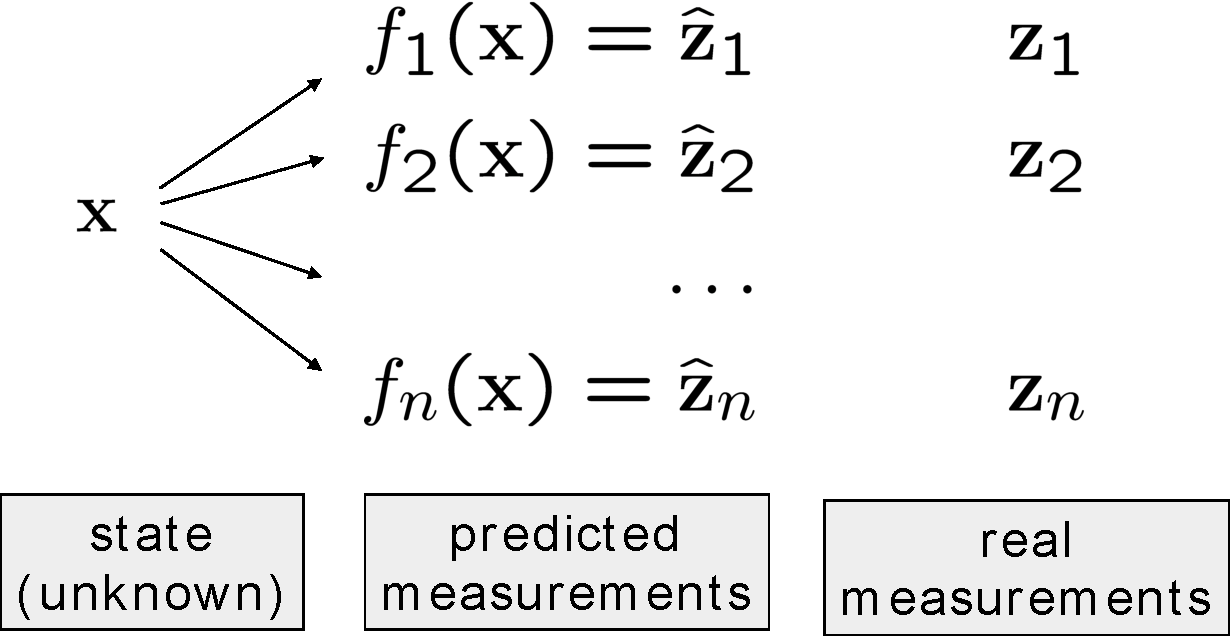
\includegraphics[width=0.7\textwidth]{images/least_squares.pdf}
    \end{center}

\end{frame}

\begin{frame}
    \frametitle{Ejemplo}
    \note{Extraído de Curso de Cyrill Stachniss https://youtu.be/r2cyMQ5NB1o?si=WYODHSkWun3FL7jR}
    
    \begin{center}
        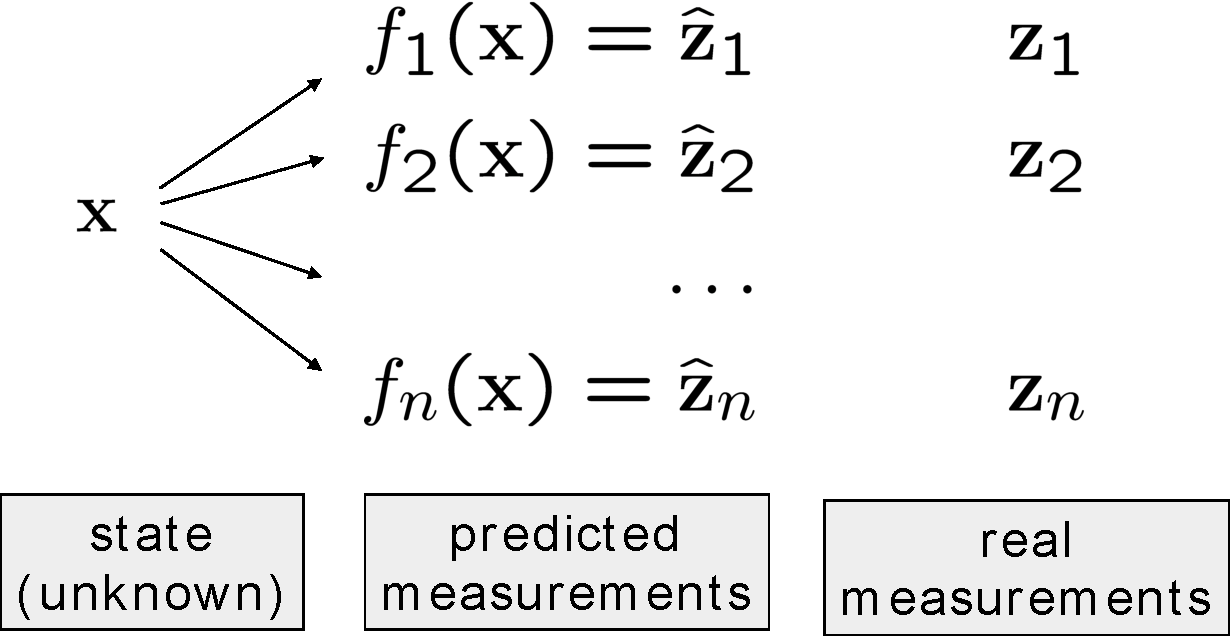
\includegraphics[width=0.7\textwidth]{images/least_squares.pdf}
    \end{center}
    
    \begin{itemize}
        \item $\stateBold$ posición de los puntos 3D
        \item $\observationBold_{i}$ coordenadas de los puntos 3D proyectados en las imágenes
        \item Estimar la posición 3D más probable de los puntos basado en las proyecciones en las imágenes (dada las poses de la cámara)
    \end{itemize}
\end{frame}

\begin{frame}
    \frametitle{Función de Error}
    \note{Extraído de Curso de Cyrill Stachniss https://youtu.be/r2cyMQ5NB1o?si=WYODHSkWun3FL7jR}
    
    \begin{itemize}
        \item El error $\error_{i}$ suele ser la diferencia entre la medición real y la predicción:
            \begin{equation*}
                \error_{i}\left( \stateBold \right) = \observationBold_{i} - f_{i}\left( \stateBold \right)
            \end{equation*}
        \item Supongamos que el error tiene una distribución normal con media cero
        \item Error Gaussiano con matriz de información $\informationMatrix_{i}$
        \item El error al cuadrado de una medición depende sólo del estado y es un escalar:
            \begin{equation*}
                \error_{i}\left( \stateBold \right) = \error_{i}\left( \stateBold \right)^{\top} \informationMatrix_{i} \error_{i}\left( \stateBold \right)
            \end{equation*}
    \end{itemize}
\end{frame}

\begin{frame}
    \frametitle{Objetivo: Encontrar el Mínimo}
    \note{Extraído de Curso de Cyrill Stachniss https://youtu.be/r2cyMQ5NB1o?si=WYODHSkWun3FL7jR}
    
    \begin{itemize}
        \item Encontrar el estado $\stateBold^{*}$ que minimiza el error dados todas las mediciones
        
        \begin{center}
            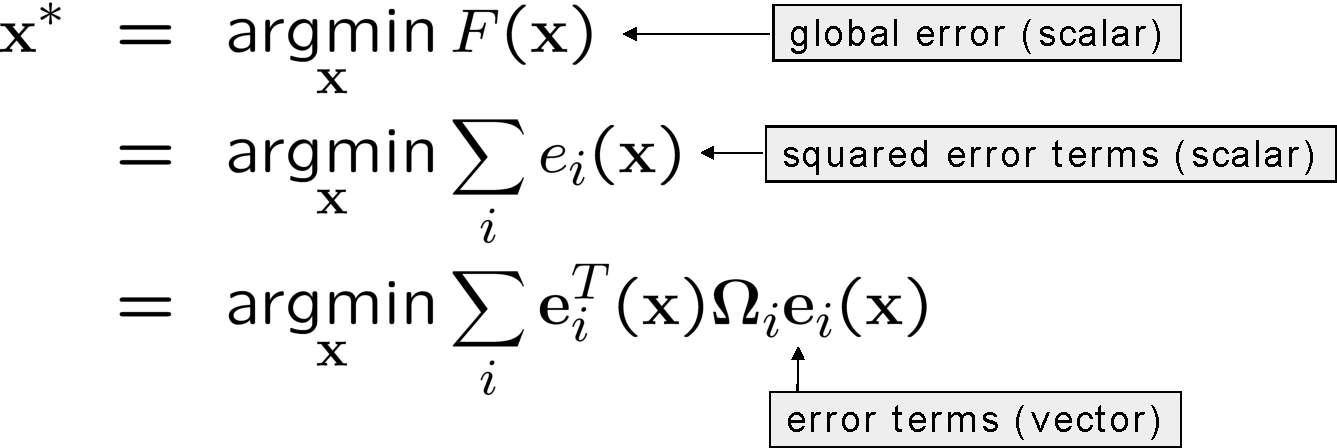
\includegraphics[width=0.7\textwidth]{images/find_minimum.pdf}
        \end{center}
    \end{itemize}

\end{frame}

\begin{frame}
    \frametitle{Objetivo: Encontrar el Mínimo}
    \note{Extraído de Curso de Cyrill Stachniss https://youtu.be/r2cyMQ5NB1o?si=WYODHSkWun3FL7jR}
    
    \begin{itemize}
        \item Encontrar el estado $\stateBold^{*}$ que minimiza el error dados todas las mediciones
        
        \begin{equation*}
            \stateBold^{*} = \argmin_{\stateBold} \sum_{i} \error_{i}\left( \stateBold \right)^{\top} \informationMatrix_{i} \error_{i}\left( \stateBold \right)
        \end{equation*}
        
        
        \item Una solución general es derivar la función de error global y encontrar sus nulos
        \item En general compleja y con solución no cerrada $\rightarrow$ Solución con Métodos numéricos
    \end{itemize}
    
\end{frame}


\begin{frame}
    \frametitle{Suposiciones}
    \note{Extraído de Curso de Cyrill Stachniss https://youtu.be/r2cyMQ5NB1o?si=WYODHSkWun3FL7jR}
    \begin{itemize}
        \item Hay una ``buena'' solución inicial disponible
        \item Las funciones de error son ``suaves'' en la vecindad del mínimo (con suerte global)
        \item Entonces, podemos resolver el problema con linearizaciones locales iterativas
    \end{itemize}

\end{frame}

\begin{frame}
    \frametitle{Resolvemos utilizando Linearizaciones locales iterativas}
    \note{Extraído de Curso de Cyrill Stachniss https://youtu.be/r2cyMQ5NB1o?si=WYODHSkWun3FL7jR}
    \begin{itemize}
        \item Linealizar los términos de error alrededor del solución actual/solución inicial
        \item Calcular la primera derivada de la función de error al cuadrado
        \item Setear en cero y resolver el sistema lineal
        \item Obtener el nuevo estado (que con suerte estará más cerca del mínimo)
        \item Iterar
    \end{itemize}
\end{frame}

\begin{frame}
    \frametitle{Linearizar la Función de Error}
    \note{Extraído de Curso de Cyrill Stachniss https://youtu.be/r2cyMQ5NB1o?si=WYODHSkWun3FL7jR}
    
    \begin{itemize}
        \item Podemos aproximar el error al rededor de una estimación inicial $\stateBold$ a través de una expansión de Taylor
    \end{itemize}
    
    \begin{equation*}
        \error_{i}(\stateBold + \vec{\Delta}\stateBold) \simeq  \underbrace{\error_{i}(\stateBold)}_{\error_{i}} + \jacobian_{i}\vec{\Delta}\stateBold \quad \text{con} \quad \jacobian_{i} = \dfrac{\partial\error_{i}(\stateBold)}{\partial\stateBold}
    \end{equation*}
    
\end{frame}

\begin{frame}
    \frametitle{Error Cuadrático}
    \note{Extraído de Curso de Cyrill Stachniss https://youtu.be/r2cyMQ5NB1o?si=WYODHSkWun3FL7jR}
    
    \begin{itemize}
        \item Con la linealización anterior, podemos fijar $\stateBold$ y llevar a cabo la minimización en los incrementos $\Delta\stateBold$
        \item Reemplazamos la expansión de Taylor en los términos de error al cuadrado:
        \only<1>{
            \begin{align*}
                \error_{i}(\stateBold + \vec{\Delta}\stateBold) &= \dots
            \end{align*}
        }
        \only<2>{
            \begin{align*}
                \error_{i}(\stateBold + \vec{\Delta}\stateBold) &= \error_{i}\left( \stateBold + \Delta \stateBold \right)^{\top} \informationMatrix_{i} \error_{i}\left( \stateBold  + \Delta \stateBold \right)
            \end{align*}
        }
        \only<3>{
            \begin{align*}
                \error_{i}(\stateBold + \vec{\Delta}\stateBold) &= \error_{i}\left( \stateBold + \Delta \stateBold \right)^{\top} \informationMatrix_{i} \error_{i}\left( \stateBold  + \Delta \stateBold \right)\\
                &\simeq \left( \error_{i} + \jacobian_{i} \Delta \stateBold \right)^{\top} \informationMatrix_{i} \left( \error_{i} + \jacobian_{i} \Delta \stateBold \right)
            \end{align*}
        }
        \only<4>{
            \begin{align*}
                \error_{i}(\stateBold + \vec{\Delta}\stateBold) &= \error_{i}\left( \stateBold + \Delta \stateBold \right)^{\top} \informationMatrix_{i} \error_{i}\left( \stateBold  + \Delta \stateBold \right)\\
                &\simeq \left( \error_{i} + \jacobian_{i} \Delta \stateBold \right)^{\top} \informationMatrix_{i} \left( \error_{i} + \jacobian_{i} \Delta \stateBold \right)\\
                &= \error_{i}^{\top} \informationMatrix_{i} \error_{i} + \error_{i}^{\top} \informationMatrix_{i} \jacobian_{i} \Delta \stateBold + \Delta \stateBold^{\top} \jacobian_{i}^{\top} \informationMatrix_{i} \error_{i} +  \Delta \stateBold^{\top} \jacobian_{i}^{\top} \informationMatrix_{i} \jacobian_{i} \Delta \stateBold
            \end{align*}
        }
    \end{itemize}
\end{frame}

\begin{frame}
    \frametitle{Error cuadrático (cont.)}
    \note{Extraído de Curso de Cyrill Stachniss https://youtu.be/r2cyMQ5NB1o?si=WYODHSkWun3FL7jR}
    
    \begin{itemize}
        \item Todos los sumandos son escalares por lo que la transposición no tiene ningún efecto
        \item Agrupando términos similares obtenemos:
        \only<1>{
            \begin{align*}
                \error_{i}(\stateBold + \vec{\Delta}\stateBold) &\simeq \error_{i}^{\top} \informationMatrix_{i} \error_{i} + \error_{i}^{\top} \informationMatrix_{i} \jacobian_{i} \Delta \stateBold + \Delta \stateBold^{\top} \jacobian_{i}^{\top} \informationMatrix_{i} \error_{i} +  \Delta \stateBold^{\top} \jacobian_{i}^{\top} \informationMatrix_{i} \jacobian_{i} \Delta \stateBold
            \end{align*}
        }
        \only<2>{
            \begin{align*}
                \error_{i}(\stateBold + \vec{\Delta}\stateBold) &\simeq \error_{i}^{\top} \informationMatrix_{i} \error_{i} + \error_{i}^{\top} \informationMatrix_{i} \jacobian_{i} \Delta \stateBold + \Delta \stateBold^{\top} \jacobian_{i}^{\top} \informationMatrix_{i} \error_{i} +  \Delta \stateBold^{\top} \jacobian_{i}^{\top} \informationMatrix_{i} \jacobian_{i} \Delta \stateBold \\
                &= \underbrace{\error_{i}^{\top} \informationMatrix_{i} \error_{i}}_{c_{i}} + 2 \underbrace{\error_{i}^{\top} \informationMatrix_{i} \jacobian_{i}}_{\linearSystemb_{i}} \Delta \stateBold + \Delta \stateBold^{\top} \underbrace{\jacobian_{i}^{\top} \informationMatrix_{i} \jacobian_{i}}_{\linearSystemH_{i}} \Delta \stateBold
            \end{align*}
        }
    \end{itemize}
    
    
\end{frame}

\begin{frame}
    \frametitle{Global Error}
    \note{Extraído de Curso de Cyrill Stachniss https://youtu.be/r2cyMQ5NB1o?si=WYODHSkWun3FL7jR}
    
\end{frame}

\begin{frame}
    \frametitle{Global Error (cont.)}
    \note{Extraído de Curso de Cyrill Stachniss https://youtu.be/r2cyMQ5NB1o?si=WYODHSkWun3FL7jR}
    
\end{frame}

\begin{frame}
    \frametitle{Quadratic Form}
    \note{Extraído de Curso de Cyrill Stachniss https://youtu.be/r2cyMQ5NB1o?si=WYODHSkWun3FL7jR}
    
\end{frame}

\begin{frame}
    \frametitle{Deriving a Quadratic Form}
    \note{Extraído de Curso de Cyrill Stachniss https://youtu.be/r2cyMQ5NB1o?si=WYODHSkWun3FL7jR}
    
\end{frame}

\begin{frame}
    \frametitle{Quadratic Form}
    \note{Extraído de Curso de Cyrill Stachniss https://youtu.be/r2cyMQ5NB1o?si=WYODHSkWun3FL7jR}
    
\end{frame}

\begin{frame}
    \frametitle{Minimizing the Quadratic Form}
    \note{Extraído de Curso de Cyrill Stachniss https://youtu.be/r2cyMQ5NB1o?si=WYODHSkWun3FL7jR}
    
\end{frame}

\begin{frame}
    \frametitle{Gauss-Newton Solution}
    \note{Extraído de Curso de Cyrill Stachniss https://youtu.be/r2cyMQ5NB1o?si=WYODHSkWun3FL7jR}
    
\end{frame}

\begin{frame}
    \frametitle{Example: Odometry Calibration}
    \note{Extraído de Curso de Cyrill Stachniss https://youtu.be/r2cyMQ5NB1o?si=WYODHSkWun3FL7jR}
    
\end{frame}

\begin{frame}
    \frametitle{Odometry Calibration (cont.)}
    \note{Extraído de Curso de Cyrill Stachniss https://youtu.be/r2cyMQ5NB1o?si=WYODHSkWun3FL7jR}
    
\end{frame}

\begin{frame}
    \frametitle{Questions}
    \note{Extraído de Curso de Cyrill Stachniss https://youtu.be/r2cyMQ5NB1o?si=WYODHSkWun3FL7jR}
    
\end{frame}

\begin{frame}
    \frametitle{How to Efficiently Solve the Linear System?}
    \note{Extraído de Curso de Cyrill Stachniss https://youtu.be/r2cyMQ5NB1o?si=WYODHSkWun3FL7jR}
    
\end{frame}

\begin{frame}
    \frametitle{Cholesky Decomposition for Solving a Linear System}
    \note{Extraído de Curso de Cyrill Stachniss https://youtu.be/r2cyMQ5NB1o?si=WYODHSkWun3FL7jR}
    
\end{frame}

\begin{frame}
    \frametitle{Gauss-Newton Summary}
    \note{Extraído de Curso de Cyrill Stachniss https://youtu.be/r2cyMQ5NB1o?si=WYODHSkWun3FL7jR}
    
\end{frame}

\begin{frame}
    \frametitle{Least Squares vs. Probabilistic State Estimation}
    \note{Extraído de Curso de Cyrill Stachniss https://youtu.be/r2cyMQ5NB1o?si=WYODHSkWun3FL7jR}
    
\end{frame}

\begin{frame}
    \frametitle{Start with State Estimation}
    \note{Extraído de Curso de Cyrill Stachniss https://youtu.be/r2cyMQ5NB1o?si=WYODHSkWun3FL7jR}
    
\end{frame}

\begin{frame}
    \frametitle{Log Likelihood}
    \note{Extraído de Curso de Cyrill Stachniss https://youtu.be/r2cyMQ5NB1o?si=WYODHSkWun3FL7jR}
    
\end{frame}

\begin{frame}
    \frametitle{Gaussian Assumption}
    \note{Extraído de Curso de Cyrill Stachniss https://youtu.be/r2cyMQ5NB1o?si=WYODHSkWun3FL7jR}
    
\end{frame}

\begin{frame}
    \frametitle{Log of a Gaussian}
    \note{Extraído de Curso de Cyrill Stachniss https://youtu.be/r2cyMQ5NB1o?si=WYODHSkWun3FL7jR}
    
\end{frame}

\begin{frame}
    \frametitle{Error Function as Exponent}
    \note{Extraído de Curso de Cyrill Stachniss https://youtu.be/r2cyMQ5NB1o?si=WYODHSkWun3FL7jR}
    
\end{frame}

\begin{frame}
    \frametitle{Log Likelihood with Error Terms}
    \note{Extraído de Curso de Cyrill Stachniss https://youtu.be/r2cyMQ5NB1o?si=WYODHSkWun3FL7jR}
    
\end{frame}

\begin{frame}
    \frametitle{Maximizing the Log Likelihood}
    \note{Extraído de Curso de Cyrill Stachniss https://youtu.be/r2cyMQ5NB1o?si=WYODHSkWun3FL7jR}
    
\end{frame}

\begin{frame}
    \frametitle{Minimizing the Squared Error is Equivalent to Maximizing the Log Likelihood of Independent Gaussian Distributions}
    \note{Extraído de Curso de Cyrill Stachniss https://youtu.be/r2cyMQ5NB1o?si=WYODHSkWun3FL7jR}
    
\end{frame}

\begin{frame}
    \frametitle{Summary}
    \note{Extraído de Curso de Cyrill Stachniss https://youtu.be/r2cyMQ5NB1o?si=WYODHSkWun3FL7jR}
    
\end{frame}

\begin{frame}
    \frametitle{Literature}
    \note{Extraído de Curso de Cyrill Stachniss https://youtu.be/r2cyMQ5NB1o?si=WYODHSkWun3FL7jR}
    
\end{frame}